\section{FlexLION}
\subsection{Target Interconnect Fabric}
The goal of our proposal FlexLION is to enable an all-to-all interconnection fabric in which each sender can dynamically allocate bandwidth to each of its output links based on an application's communication demand.\\
In an all-to-all network without configuration capability (as shown Figure~\ref{fig:logtopawgr}), each input port communicates with each output port with the same link bandwidth (for instance, a standard AWGR as in Figure~\ref{fig:awgrmatrix} provides such a fabric).
\begin{figure*}[t!]
    \centering
        \begin{subfigure}[t]{0.31\linewidth}
        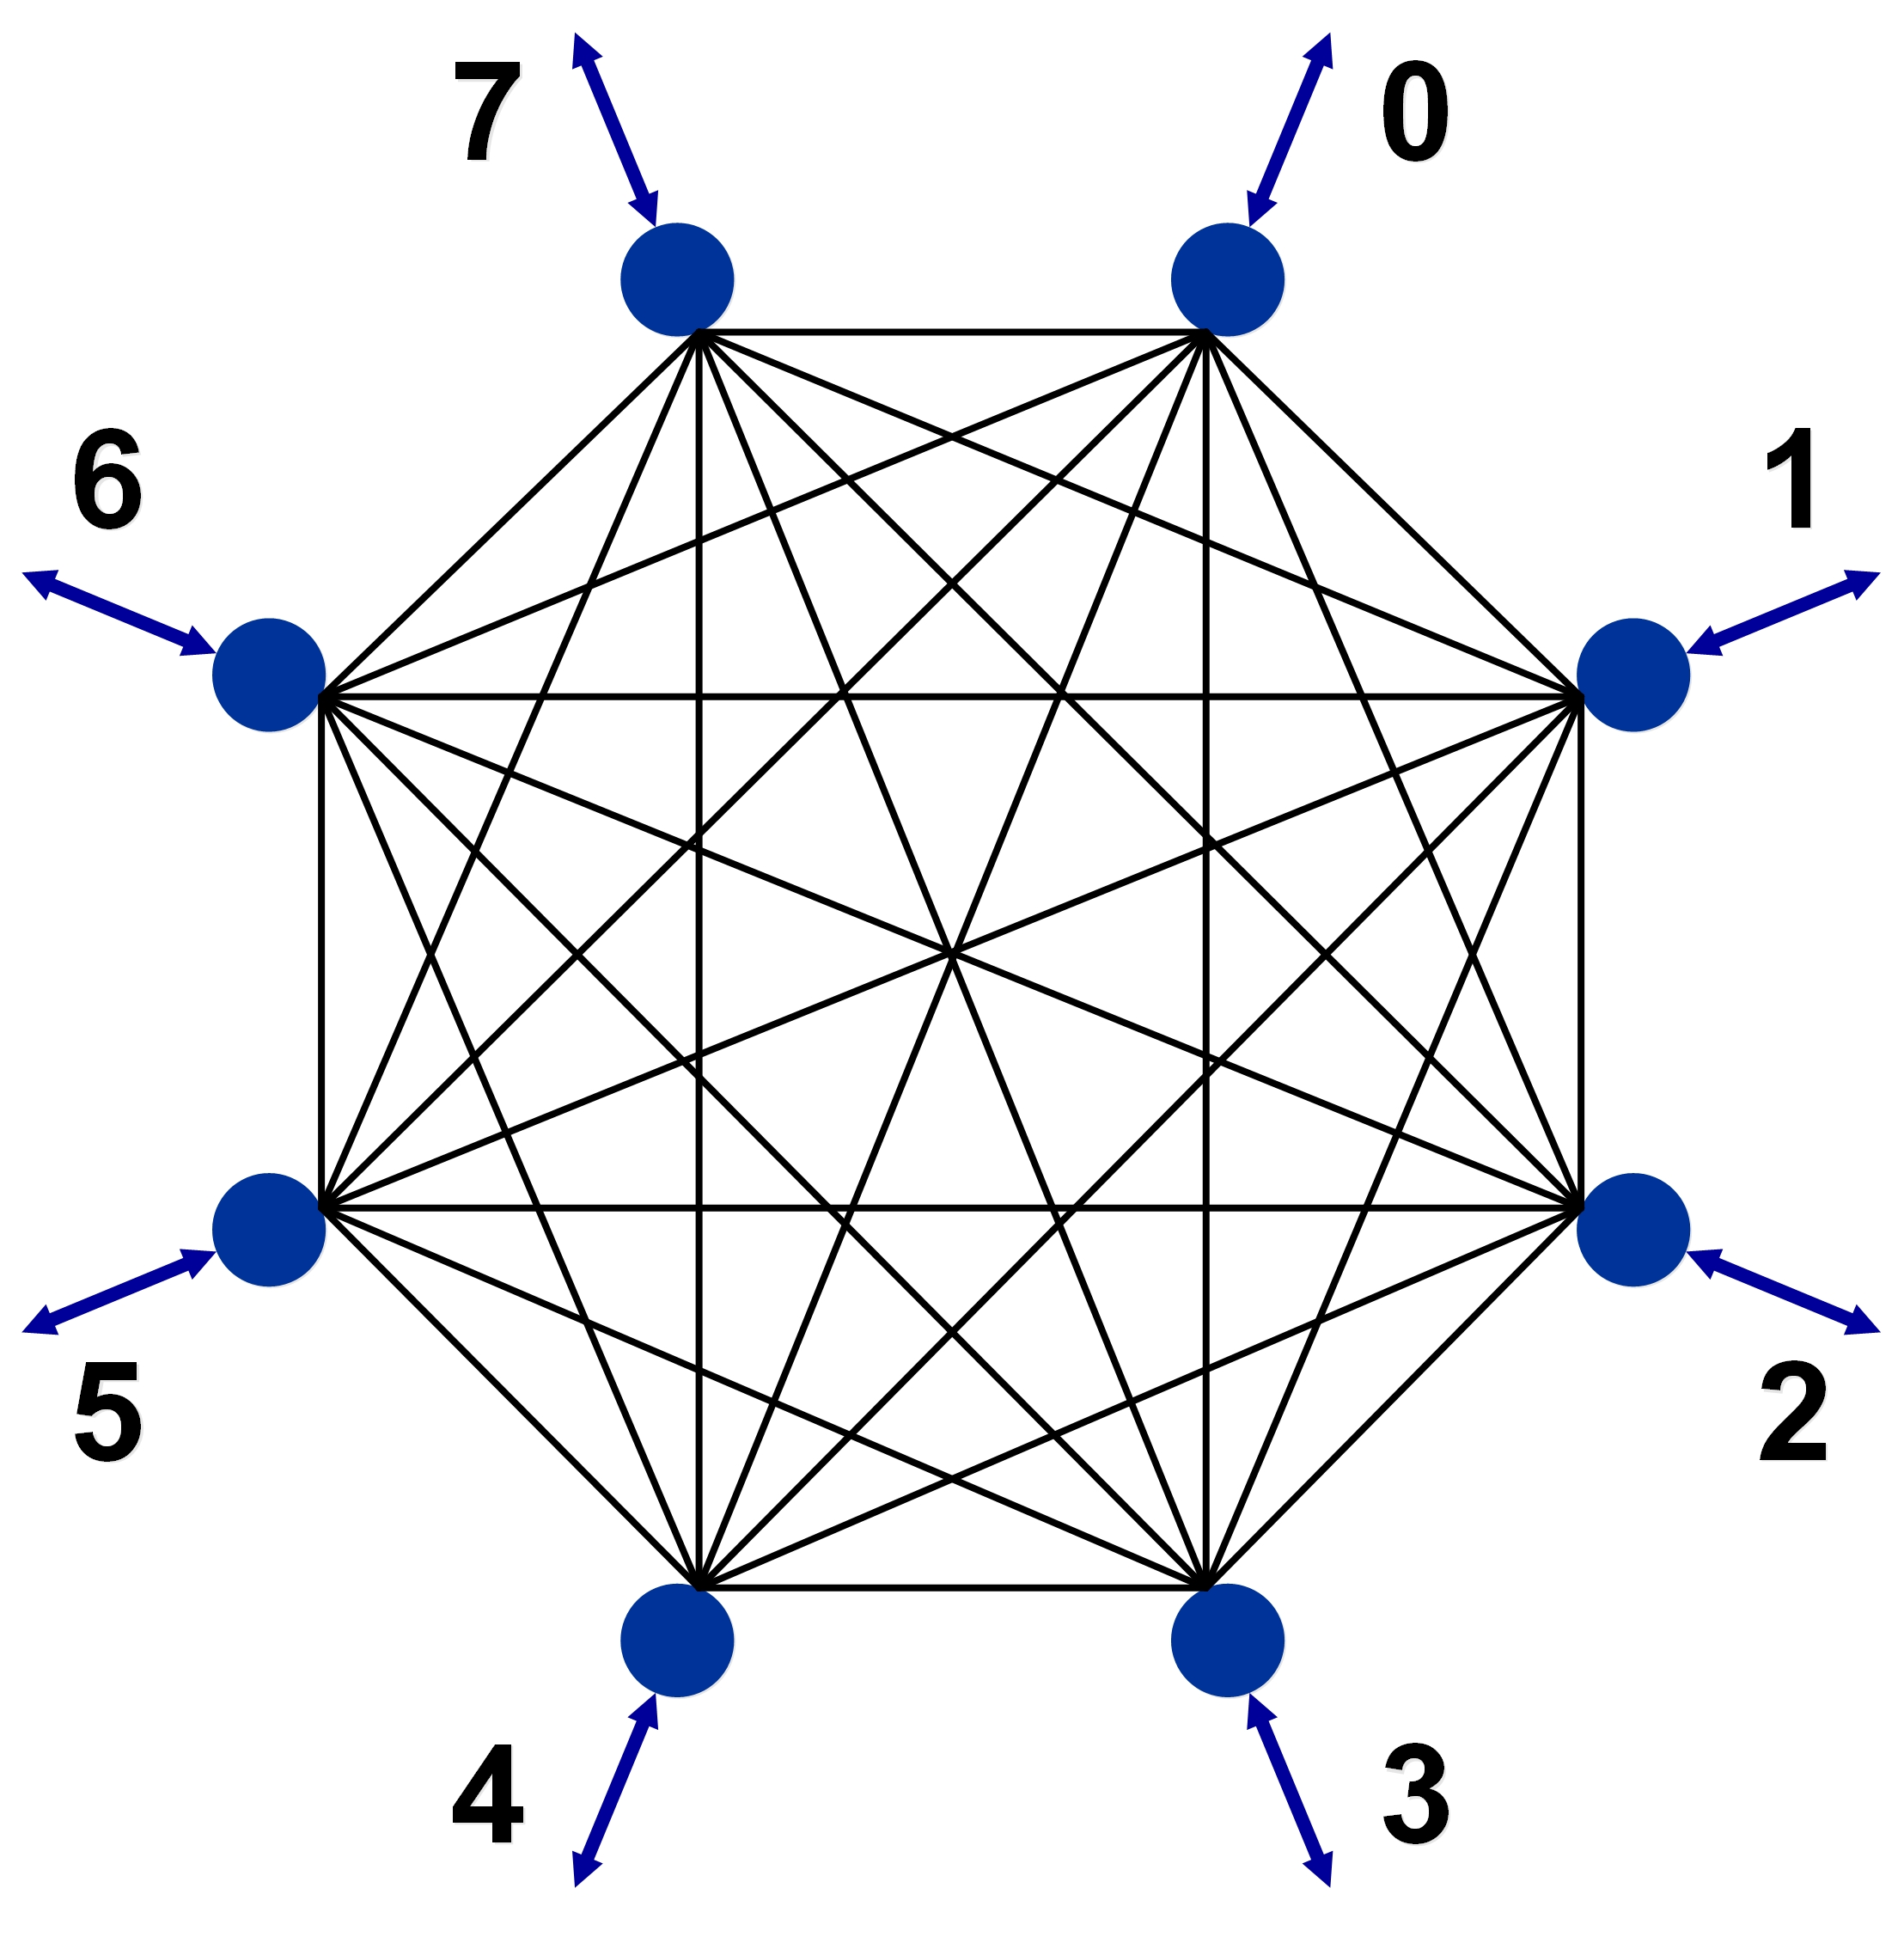
\includegraphics[width=\textwidth, clip]{Figures/logtopawgr.jpg}
        \caption{All-to-all network with uniform link bandwidth and no reconfiguration}
        		\label{fig:logtopawgr}
       \end{subfigure}
        \hspace{0.1cm}
        \begin{subfigure}[t]{0.31\linewidth}
        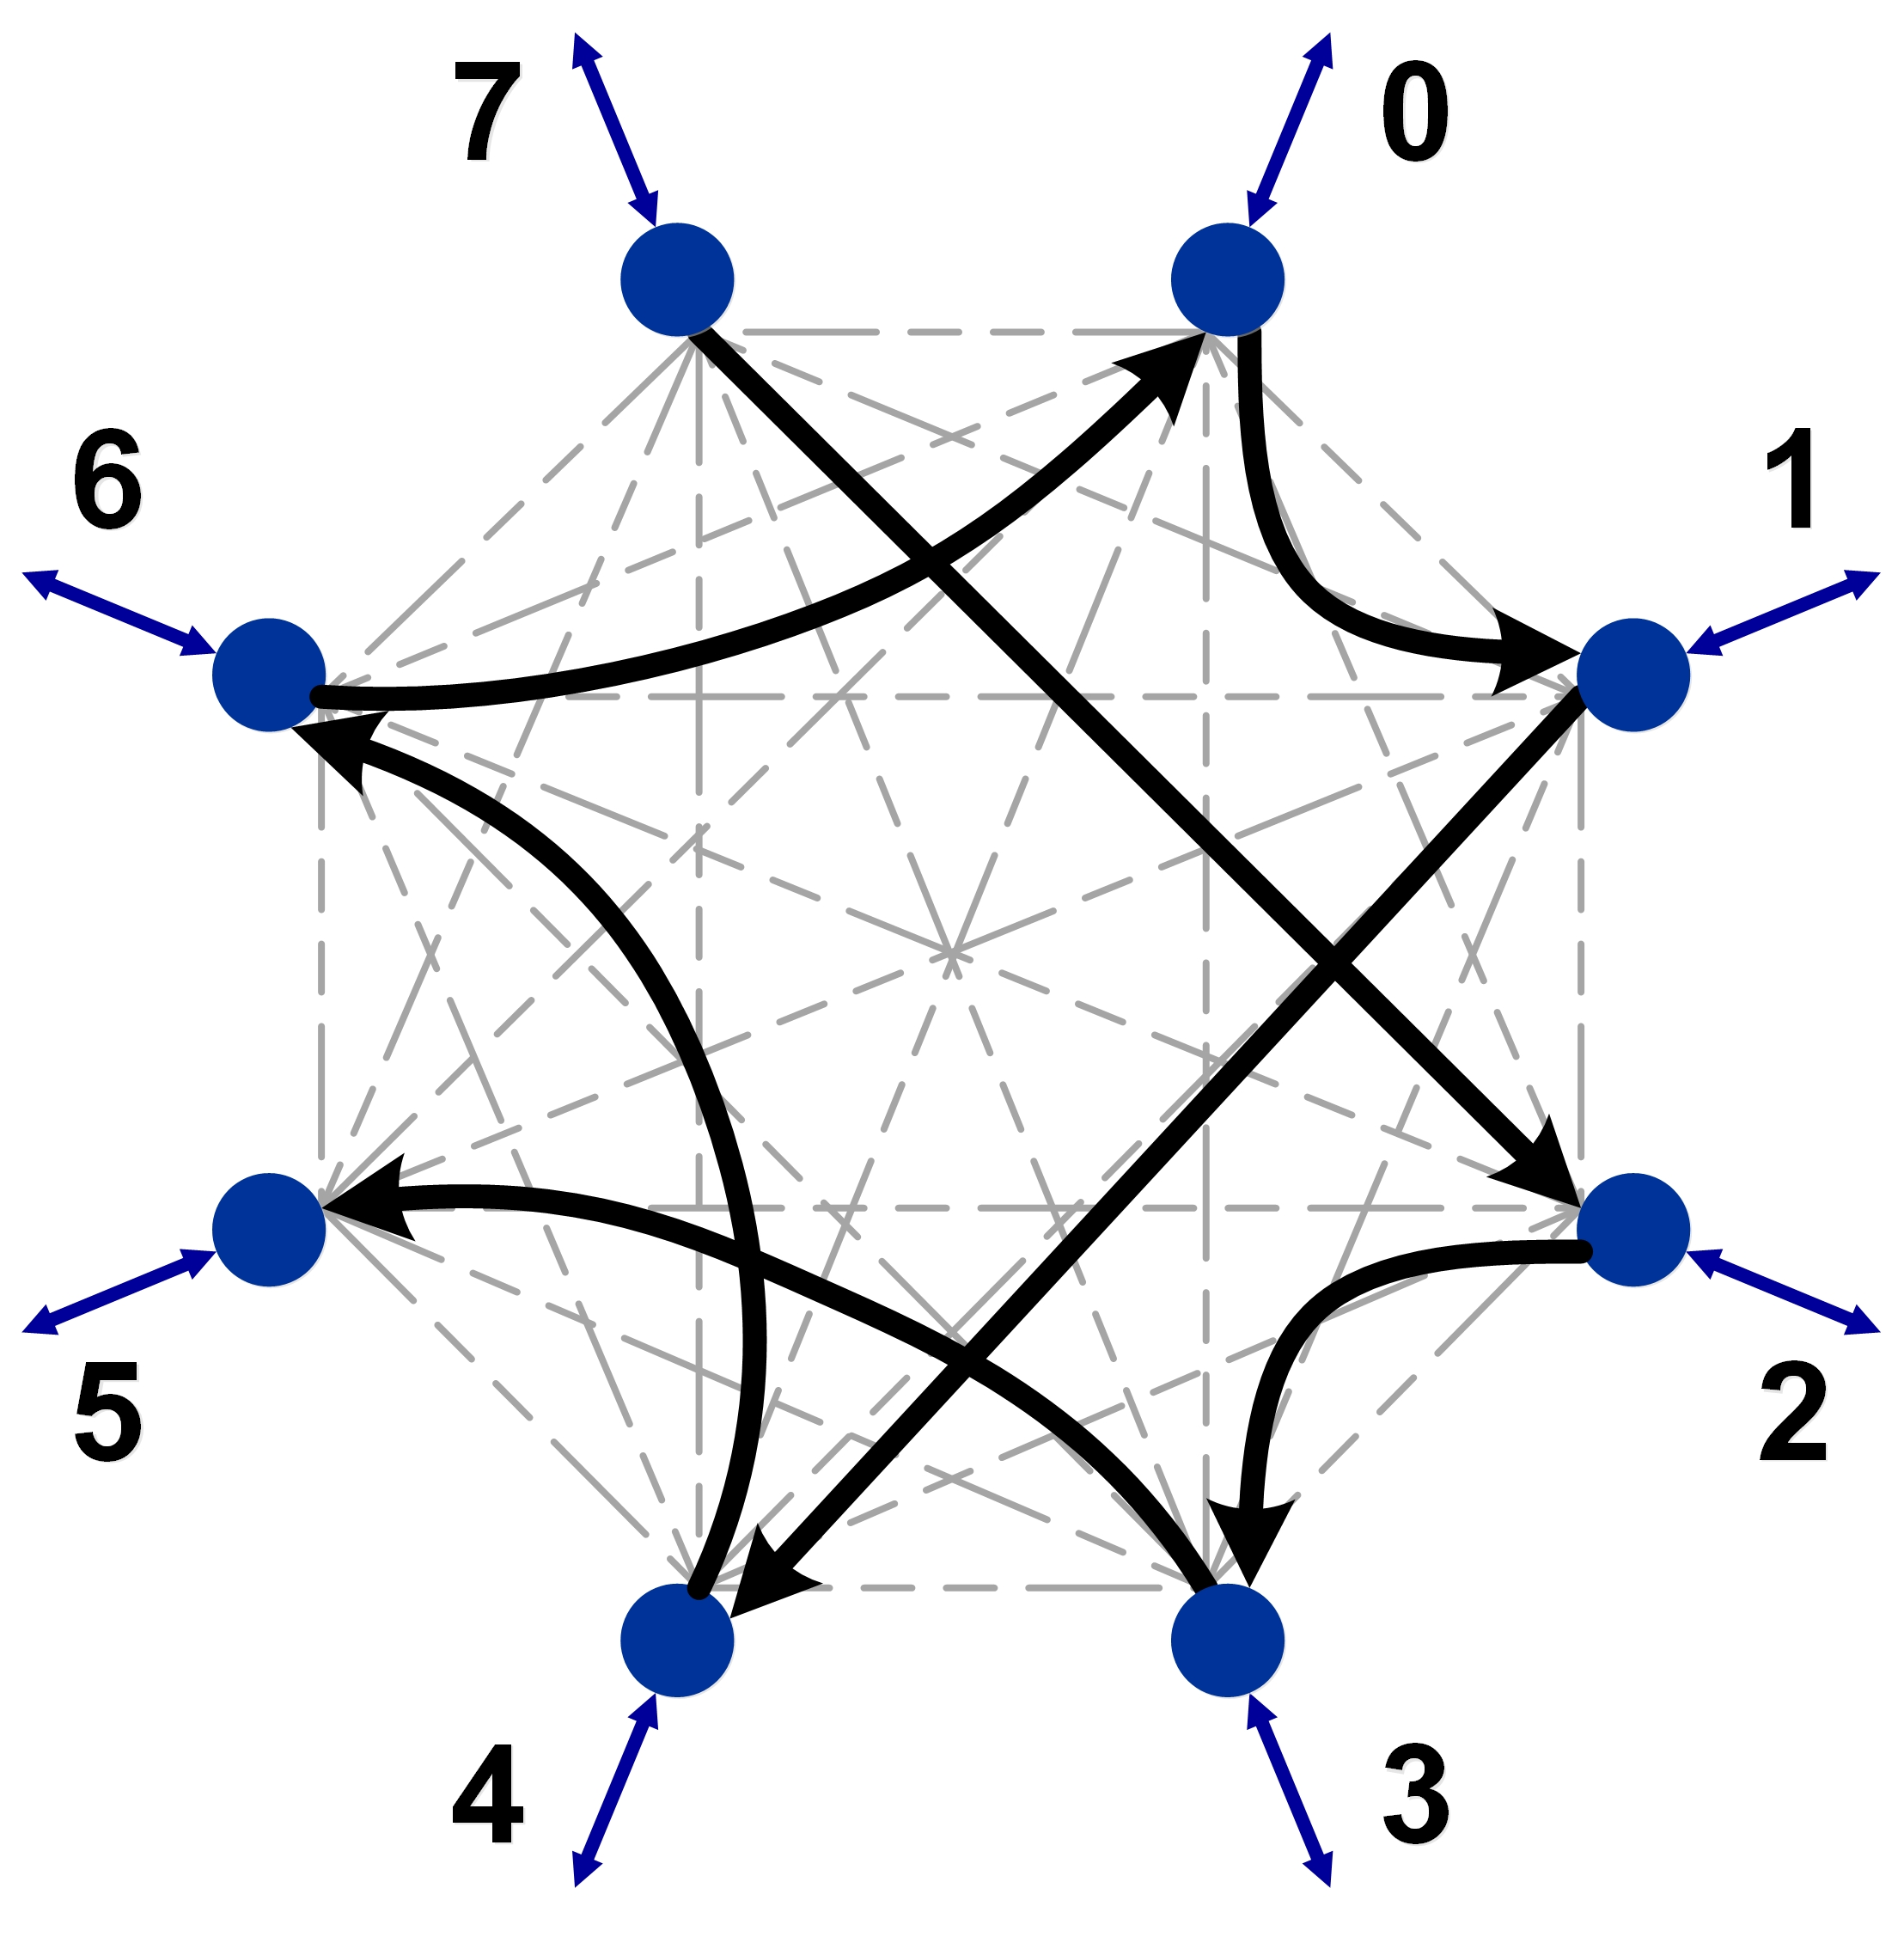
\includegraphics[width=\textwidth, clip]{Figures/logtopmems.jpg}
        \caption{Circuit-switched crossbar. Each sender can only send to one receiver using the entire available bandwidth; all other links are disconnected.}
        		\label{fig:logtopmems}
    \end{subfigure}
        \hspace{0.1cm}
    \begin{subfigure}[t]{0.31\linewidth}
        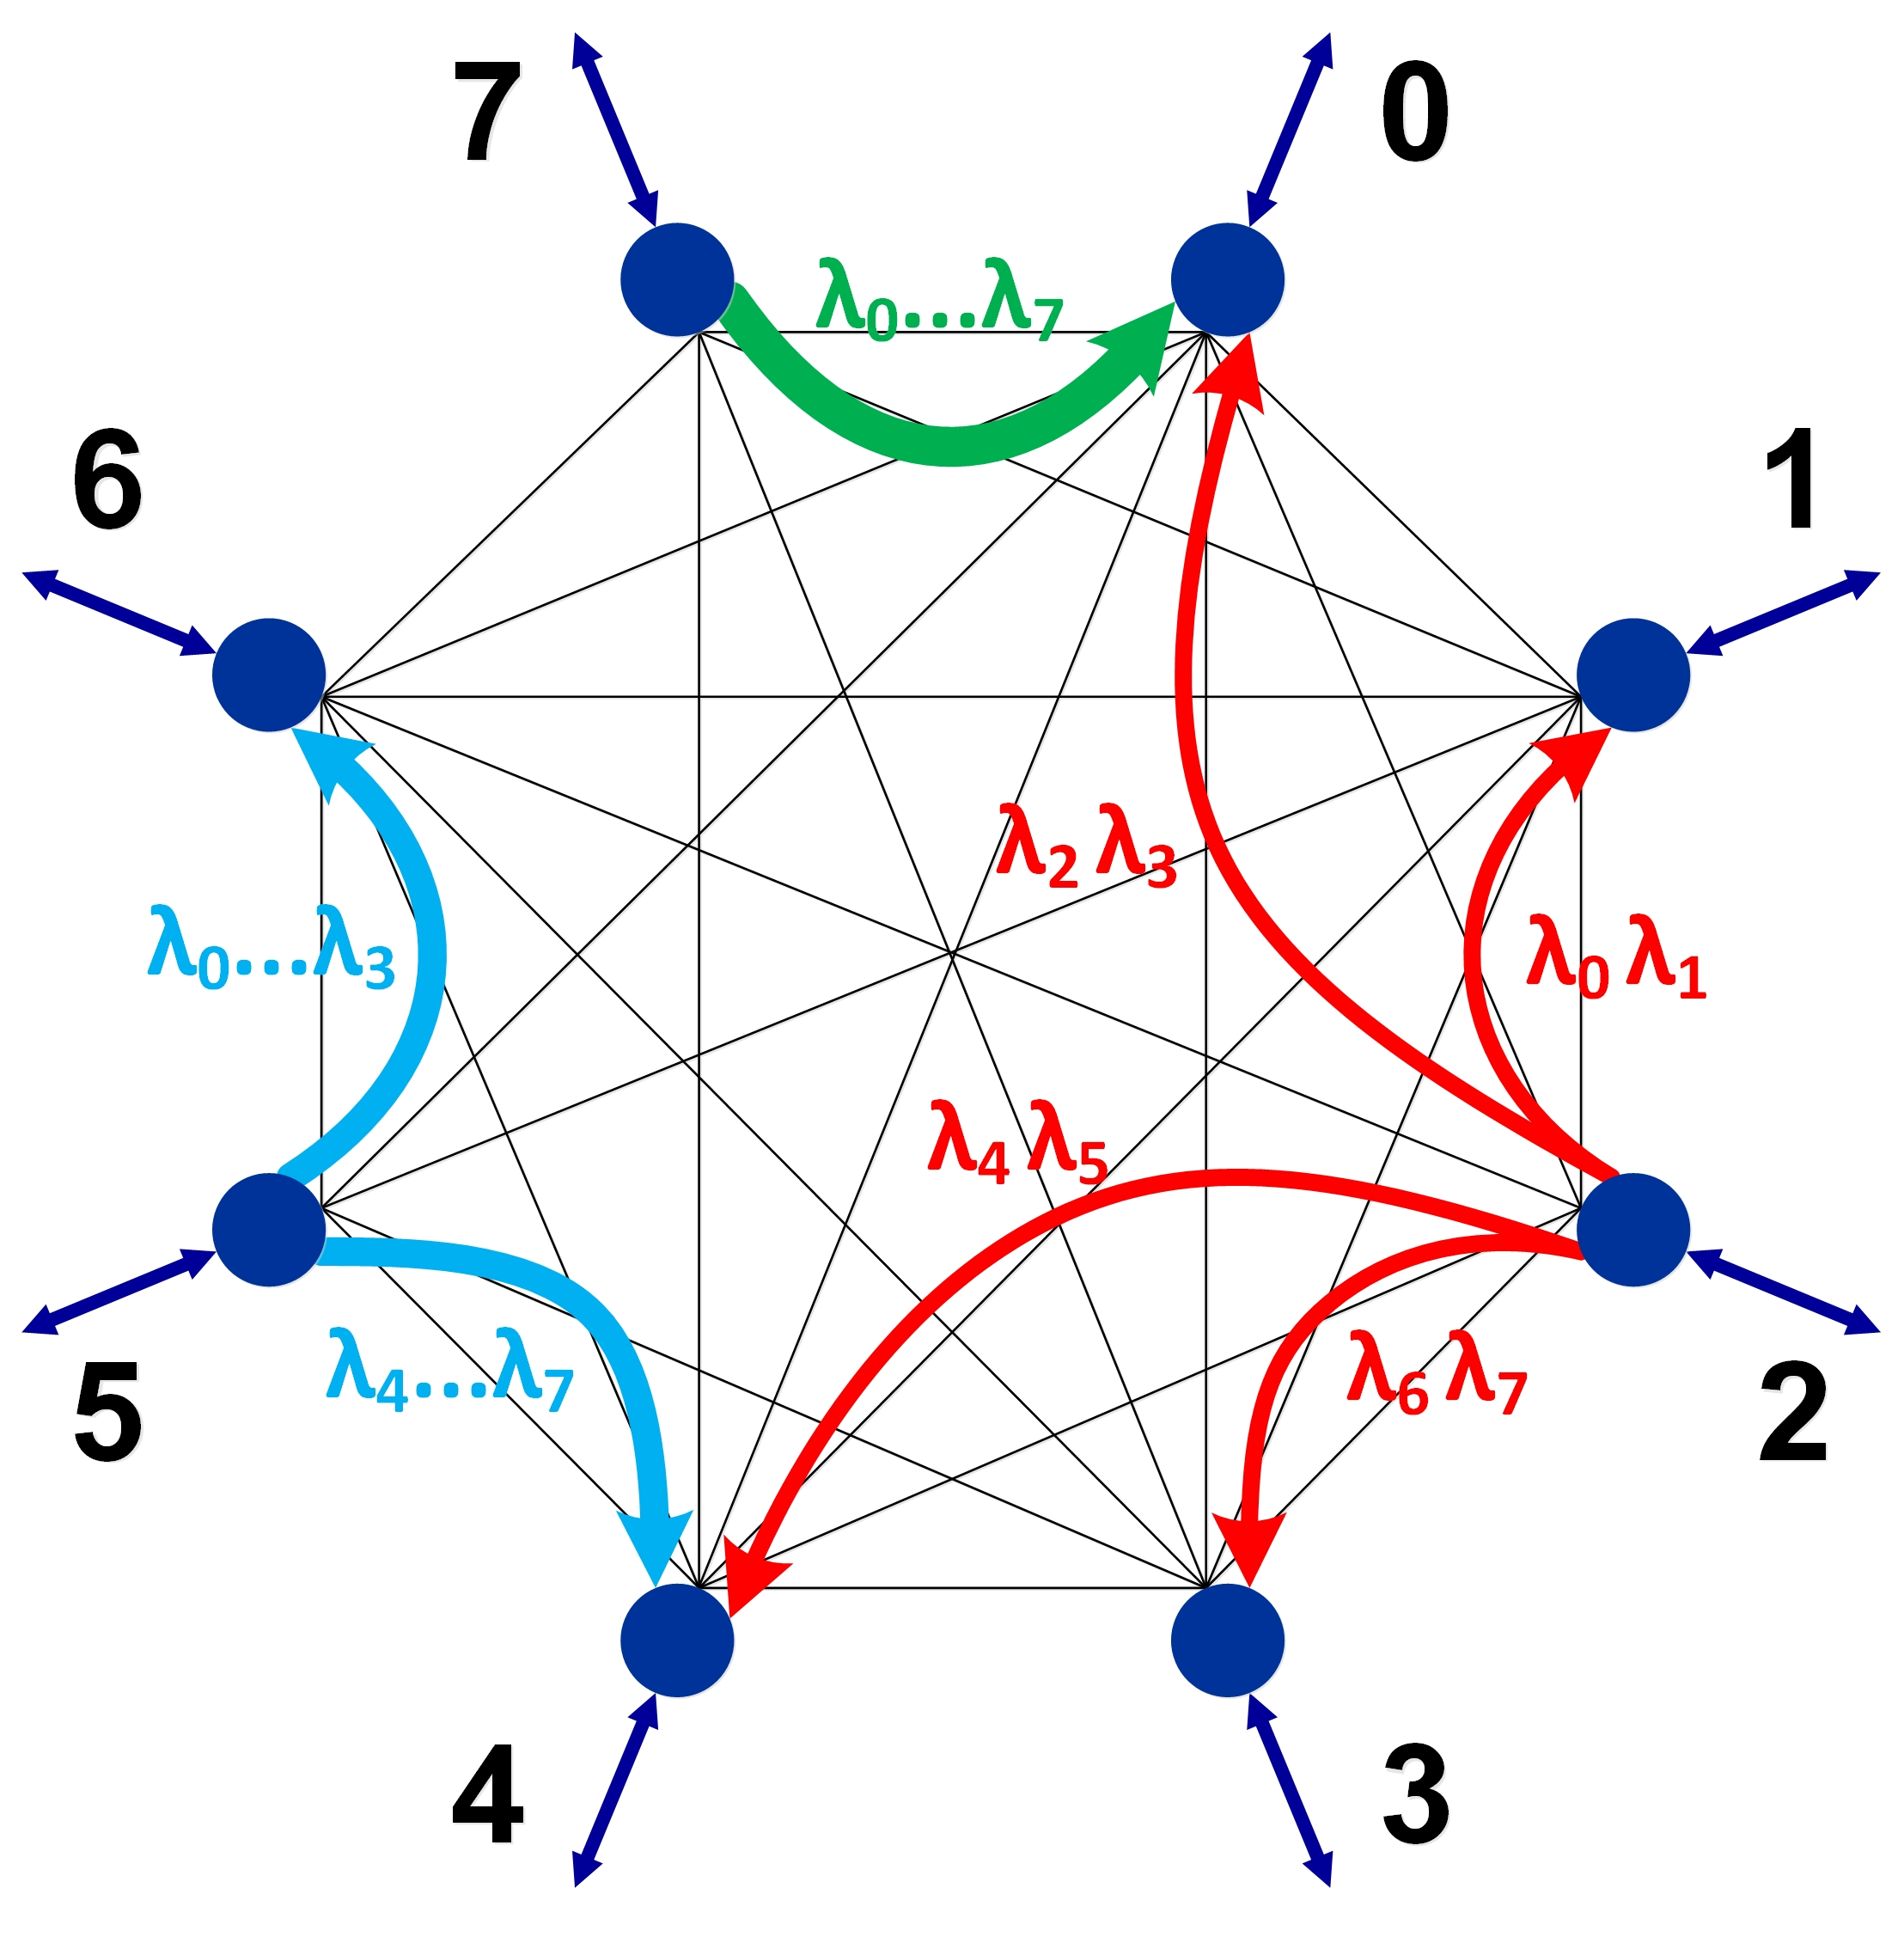
\includegraphics[width=\textwidth, clip]{Figures/logtopflex.jpg}
        \caption{All-to-all network with flexible bandwidth reconfiguration. Each available wavelength can be allocated to any link based on traffic demands.}
        		\label{fig:logtopflex}
    \end{subfigure}
    \caption[]{Logical all-to-all network topologies with different bandwidth reconfiguration capabilities}
\end{figure*}
Although all-to-all networks have the advantage of being a diameter-1 topology (and, in turn, offer minimal zero load latency), the bandwidth utilization in such networks is typically poor, leading to much of the network bandwidth and power being wasted on barely-utilized links. \\

This limitation can be overcome by exploiting WDM and wavelength-selective routing in SiPh components (instead of using independent all-to-all physical links between each sender-receiver pair). By leveraging this approach, each sender can have a pool of wavelengths available for data communication provided from a multi-wavelength laser and can allocate wavelengths to destinations based on the communication demands during an application. This allocation can be done by reconfiguring the optical network fabric, i.e.\ configuring which wavelengths are routed to which destinations, prior to executing a workload.\\
Previous proposals exploited wavelength routing by either using MEMS~\cite{seok2016highly} or broadband ring resonators~\cite{bergman2014photonic} to reconfigure the network; however, both approaches are based on broadband, color-blind SiP switching elements and can only route \textit{all} wavelengths from one node to another--effectively executing a circuit-switching mechanism allowing only point-to-point communication while all remaining connections are disconnected. This is illustrated in Figure~\ref{fig:logtopmems}. \\
Although these previous approaches might be useful in some scenarios (e.g., assigning all of the bandwidth to one destination to support large `elephant' flows in data centers~\cite{Farrington2010Helios}), in the vast majority of cases, traffic is more distributed and irregular in nature where one would still like to maintain connectivity to other nodes. In fact, superior performance metrics can be achieved if bandwidth reconfiguration would be more flexible and could support finer granularity between any sender-receiver pair. For instance, if a node A has to send 90\% of its traffic to node B and 10\% to node C (while other nodes are not communicated with) and have a pool of 10 wavelengths available, it would ideally allocate 9 wavelengths to node B and 1 to node C to achieve the highest performance. This could be enabled by reconfiguring the interconnection fabric to route 9 wavelengths from node A to node B and one wavelength to node C. This approach reduces the number of utilized fibers, can keep all nodes communicating with each other connected at all times, provides a higher degree of freedom for reconfiguring bandwidth compared to DVFS and could even be used in combination with DVFS for further variability. An example of a reconfigured network is shown in Figure~\ref{fig:logtopflex} in which multiple links have different numbers of wavelengths (and thus bandwidth) available for communication. FlexLION provides such a switching fabric, which will be introduced in the following. 

\subsection{FlexLION: Structure and Components}
*****TODO adjust *****\\
Therefore, we assume that ASIC switches are connected to FlexLIONS and use it as the communication fabric. In our design proposal, each switch ASIC is integrated on the same package as SiP transceivers, both placed and interconnected through an active SiP interposer, yielding tight integration and high energy efficiency (e.g., Intel's state-of-the-art 100G SiP transceivers require 35pJ/bit~\cite{intelsip}, while the recently demonstrated, tightly-integrated transceivers used in our study merely consume 0.55pJ/bit at 14nm~\cite{li201525}). Optical fibers connected to the SiP transceivers from each ASIC switch are coupled in and out of the die containing the FlexLIONS fabric, enabling all-to-all communication between all connected switches. The design in Figure~\ref{fig:flexdesign} envisions to place both the switch ASICs and FlexLIONS on the same board; however, since communication is optical and thus virtually distance-independent (in terms of latency and energy), system designers have a lot of freedom in placing the switches and are not restricted to mounting them on the same board.  \\
The FlexLIONS die contains the switching fabric that enables full connectivity between each input and output port and allows for maximum flexibility in bandwidth assignment. The AWGR provides all-to-all connectivity while the MRs and MEMS switching elements are utilized for the bandwidth reconfiguration. The most efficient and suitable approach for integrating all components within the same package is to use an active optical interposer. FlexLIONS easily fits on a 156$mm^2$ ($12mm \times 13mm$) interposer, a size that is readily available (for instance from AIM Photonics~\cite{aim}. In the following, we will describe the bandwidth reconfiguration mechanism in FlexLIONS. 

\subsection{Reconfiguration Mechanism}
Figure~\ref{fig:reconfexample} shows an example configuration of a 4-node FlexLION. 
\begin{figure*}[t!]
        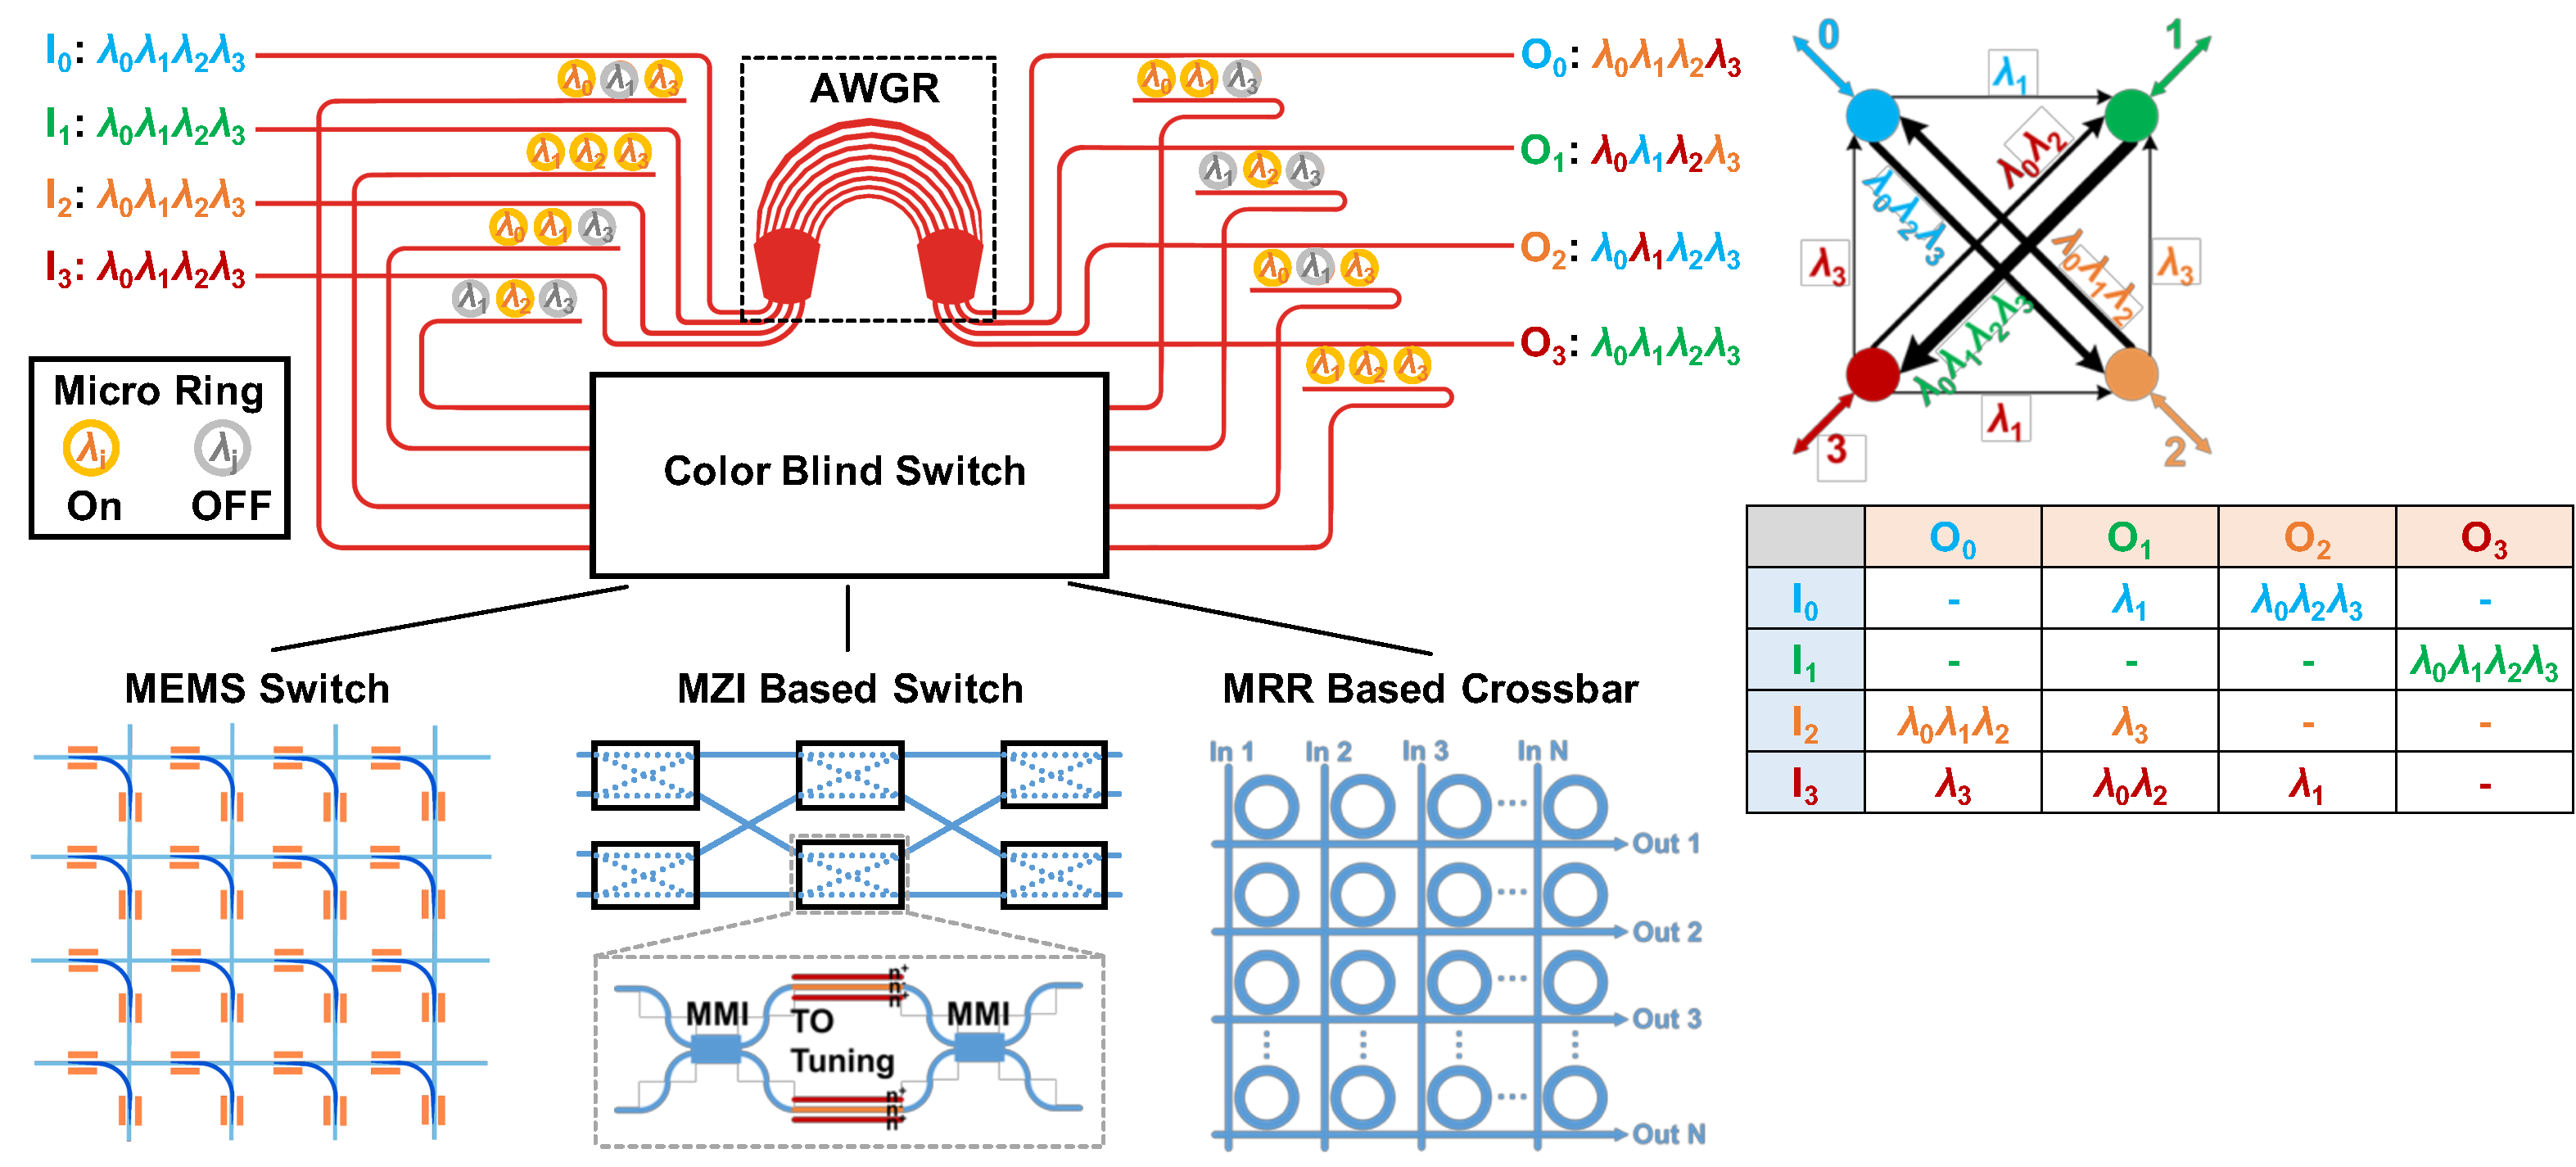
\includegraphics[width=\textwidth, clip]{Figures/reconf_example.pdf}
        \caption{Example of FlexLION reconfiguration functionality based on a $4\times4$ network.}
        		\label{fig:reconfexample}
\end{figure*}
The bandwidth reconfiguration is illustrated both in the logical topology in the top right corner and in the connectivity matrix in the bottom right corner. In all cases, the MRRs at the input and output waveguides, as well as the switching elements in the color-blind switch must be either turned ON or OFF, depending on what wavelength a sender wants to send to the destination node. Essentially, there are three different configuration cases: \\
1) A sender wants to evenly distribute its traffic (and thus the wavelengths/bandwidth) to all destination receivers. In this case, all MRRs at the input waveguide are turned OFF so that all wavelengths of the incoming WDM signal route through the AWGR, which evenly distributes the wavelengths to each output port (as described in Section~\ref{sec:awgr}). \\
2) A sender only wants to send all its traffic to the same destination: in this case, all MRRs at the input waveguide must be turned ON as they will then drop the wavelengths to the spatial switch. The adiabatic couplers in the MEMS responsible for steering wavelengths to the output port corresponding to the receiver must be turned ON (remember that the switching elements inside the MEMS are color-blind and thus always drop all wavelengths). Subsequently, the MRs at the output waveguides must be turned ON to drop the wavelength to the desired output port. This is illustrated in Figure~\ref{fig:reconfexample} from input $I_1$ to output $O_1$.  \\
3) A sender has different traffic demands for different destination nodes (see Figure~\ref{fig:reconfexample} $I_0->O_1$/$O_2$, $I_2->O_0$/$O_1$, $I_3->O_0$/$O_1$/$O_2$). In that case, there are two possibilities: either the AWGR routes a wavelength to the desired output port, in which case the MRR at the input waveguide must be turned OFF to allow the signal to go through the AWGR. Otherwise, the MRRs at the input waveguides corresponding to the wavelengths destined to the output waveguide must be turned ON in combination with the correct switching elements of the color-blind switch and the MRRs at the output waveguides. \\
Note that a reconfigurable fabric like FlexLION has one input link/fiber and one output link/fiber to each node in the network. Given that each node has only one input port, the wavelength assignment/reconfiguration must occur so that two or more senders cannot send to the same destination node on the same wavelengths (to avoid destructive interference when two signals on the same wavelength arrive at a receiver simultaneously). Therefore, such a switching fabric, though providing all-to-all connectivity, does not represent a strict point-to-point, contention-less topology, and a reconfiguration mechanism must take into account all senders, receivers, and bandwidth demands to assign wavelengths to senders while preventing destructive interference. 
\subsection{Reconfiguration from a System Perspective}
This paper proposes a novel interconnection fabric providing reconfiguration capability with compact footprint at low loss and heating requirements; however, we acknowledge that from a system perspective, performing reconfiguration is an important research area on its own and deserves detailed attention--especially as arbitrating HPC networks becomes increasingly complex as they scale up. \\
Several previous works have studied the challenge of efficiently reconfiguring an interconnection fabric in HPC system. Most notably, Bergman's research group has put much focus on developing a system with the required hardware and software to reconfigure the interconnection of a SiPh switch~\cite{shen2018software}~\cite{shen2017software}~\cite{shen2018autonomous}~\cite{shen2018accelerating}~\cite{bahadori2018design}. In particular, they successfully demonstrated a testbed system based on preconfigured FPGAs which are on the one side connected to the SiPh switch via a Digital-to-Analog converter (DAC) (which controls the MRRs via hard-coded voltage/current levels to tune the MRRs to respond to certain wavelengths) and on the other side to a central SDN controller that controls the routing tables of the electronic switches through the OpenFlow protocol~\cite{shen2018accelerating}. This traffic-driven approach oversees a switches input queues and reconfigures of the SiPh switch in a synchronised fashion to control the flow of packets while reconfiguring the physical topology. \\
This testbed performs reconfiguration of the entire control plane in 224$\mu$s and the communication between the SDN-FPGA controllers and SDN-electrical switch (223$\mu$s~\cite{shen2018software}), which occurs over a 1G Ethernet, represent the performance bottleneck. The actual reconfiguration/tuning of the SiPh components in the optical switch merely take 12$\mu$s (most of which due to the slow sub-MHz sampling speed of the DAC and the fact that the DAC is on a separate board)~\cite{shen2018software}. \\
While Bergman's work has high significance as it is the first to demonstrate a working system with a SiPh switch, much of the reconfiguration time could probably be significantly reduced by co-integrating the FPGA controller, DAC, and SiPh components in the same package (rather than on different boards), using faster sampling speeds for the DAC, using SiPh transceivers rather than 1G Ethernet for SDN-FPGA controller communication, or performing reconfiguration based a priori knowledge about a workloads communication patterns (rather than using OpenFlow). Regardless of the challenges, we point out that the reconfiguration of the SiPh components (be it MRRs, MZIs, or MEMS) are not on the critical path in terms of reconfiguration latency. 

\subsection{Utilization in HPC Center Network}
We study the impact FlexLION can have on inter-rack networks. The vast majority of high-performance data center networks are based on tree-based topologies, most prominently fat trees or clos topologies~\cite{kachris2012survey}, as they provide good scalability and load balancing properties. To save resources and power, or to adapt to current network utilization, oversubscription is a technique often used in tree-based networks in which the next tree stage only has a fraction of output links/bandwidth of the previous stage. \\
Figure~\ref{fig:networktopologies} illustrates example topologies supporting 256 nodes~\footnote{Note that the number of nodes supported by a HPC center network can vary based on the system scale. As a reference, Intel's Omni-path Director Class switches support either 192 or 768 port units~\cite{inteldir}.} comparing an HPC center network with FlexLIONS to legacy fat tree based topologies. 
\begin{figure*}[t!]
    \centering
        \begin{subfigure}[t]{0.28\linewidth}
        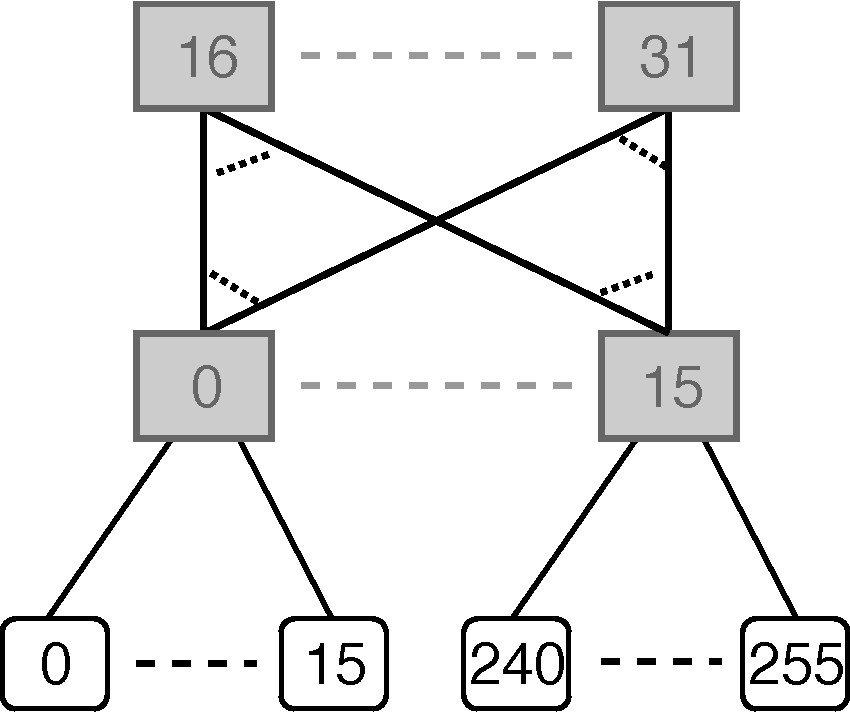
\includegraphics[width=\textwidth, clip]{Figures/treeFull.pdf}
        \caption{}
        		\label{fig:treeFull}
    \end{subfigure}
        \hspace{0.5cm}
    \begin{subfigure}[t]{0.28\linewidth}
        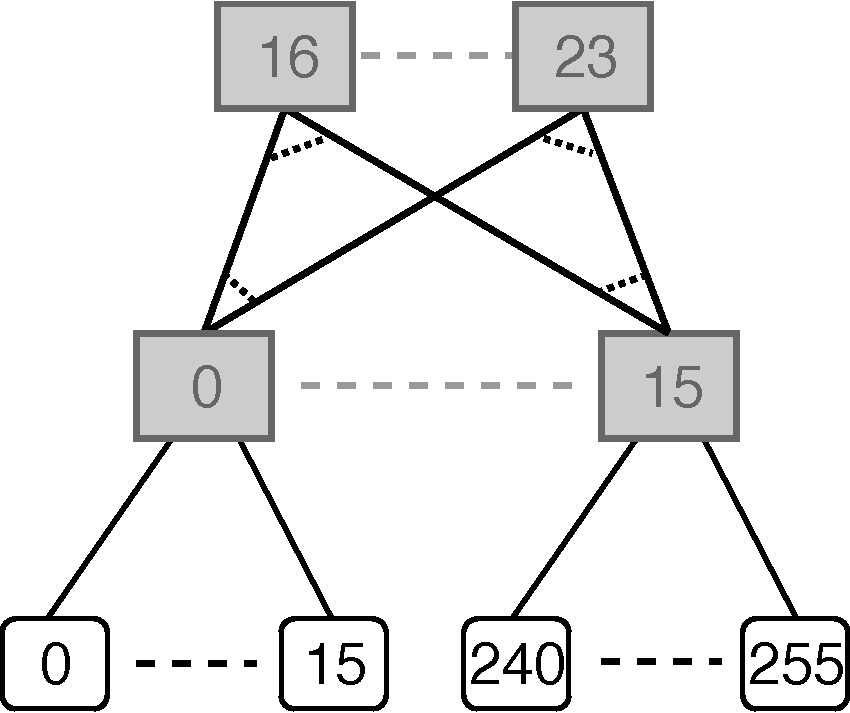
\includegraphics[width=\textwidth, clip]{Figures/treeHalf.pdf}
        \caption{}
        		\label{fig:treeHalf}
    \end{subfigure}
    \hspace{0.5cm}
    \begin{subfigure}[t]{0.28\linewidth}
        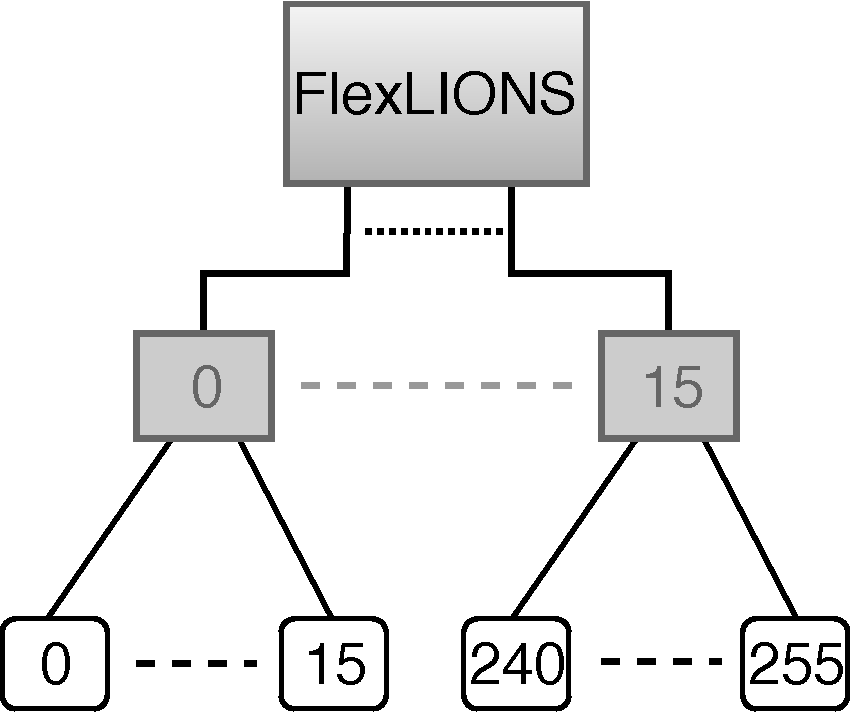
\includegraphics[width=\textwidth, clip]{Figures/flexlionIncenter.pdf}
        \caption{}
        		\label{fig:flexlionIncenter}
       \end{subfigure}
    \caption[]{HPC network topologies supporting 256 nodes: (a) Fat Tree, (b) Fat Tree with oversubscription of 2, (c) FlexLIONS}
    \label{fig:networktopologies}
\end{figure*}
Figure~\ref{fig:treeFull} depicts a 2-layer fat tree (`Fat Tree') without oversubscription, consisting of 32 32-port switches and 640 transceivers. Figure~\ref{fig:treeHalf} shows the same network, but with an oversubscription of two (`Fat Tree 2:1'), i.e.\ the number of switches on the second layer and thus the number of outgoing links on the first layer is half of that of a full Fat Tree. Figure~\ref{fig:flexlionIncenter} shows a 256-node HPC network with FlexLION, which requires 16 32-port switches, 512 transceivers, and the FlexLION fabric. 32-port switches are widely deployed and commercially available by vendors like Mellanox or Intel~\cite{mellanox}~\cite{intelomnipath}. Note that classic fat trees in HPC networks typically consist of three layers (edge, aggregate, and core switches); however, for our 256-node study we hypothesize that a 2-layer fat tree suffices to satisfy the bandwidth demands and provides more competitive zero load latency compared to the 1-layer FlexLION based network. A comparison of the properties of these three networks is listed in Table ~\ref{tab:properties}. \\
\begin{table}[]
\caption{Resource requirements of the HPC networks under investigation}
\label{tab:properties}
\centering
\begin{tabular}{@{}c|ccc@{}}
\toprule
                  & Fat Tree & Fat Tree 2:1 & FlexLIONS \\ \midrule
\#Switches     & 32       & 24           & 16        \\
\#Transceivers & 1024     & 640          & 512       \\
Link data rate & 100G     & 100G         & 100G      \\
Bisection BW   & 25.6Tb   & 12.8Tb       & 25.6Tb   \\ \bottomrule
\end{tabular}
\end{table}
One main benefit of FlexLION is that its reconfiguration capability can make efficient use of the available bandwidth and might thus provide satisfactory performs metrics without requiring a multi-stage network like trees for load balancing. In HPC center networks, the latency imposed by additional hops through a switches can have a significant impact on system performance. For instance, the most competitive design in terms of latency currently available is Intel's Omni-path ASIC switch which requires 100ns for switch traversal~\cite{intelomnipath}. With this value, the FlexLION network would reduce zero load latency from 300ns to 200ns compared to a two stage tree, which can be significant, especially in low utilization phases where the bandwidth is not stressed. Moreover, FlexLION reduces the total number of required switches and transceivers, while providing similar bisection bandwidth. In  Section 4, we will evaluate whether the bandwidth reconfiguration of FlexLION indeed allows similar performance as tree-based networks while significantly reducing resources, power, and zero load latency. 

\subsection{Design Considerations and Scalability}
The previous examples introducing FlexLION were based on four wavelengths per input port--one for each output port. The comparison in Table~\ref{tab:properties} is based on 100Gb/s per link since this is a common data rate for state-of-the-art HPC interconnects (e.g., Intel's SiP transceiver offers 100Gb/s data rate (4 wavelengths at 25Gb/s modulation rate)~\cite{intelsip}. Since data rates around 25Gb/s modulation rate offer the highest energy efficiency, FlexLION must be able to support multiple wavelengths (in this example, 4) for each receiver to support 100Gb/s communication on each link. In order to support bit-level parallelism of 4, we exploit the cyclic dependence of MRRs' resonant wavelengths and AWGRs and provide each sender with the wavelengths: $\lambda_{0}$, $\lambda_{0+FSR}$, $\lambda_{0+2*FSR}$, $\lambda_{0+3*FSR}$, ...$\lambda_{n}$, $\lambda_{n+FSR}$, $\lambda_{n+2*FSR}$, $\lambda_{n+3*FSR}$. For a 16-port FlexLIONS, each input port must be provided with $16 \times 4 = 64$ wavelengths. \\
The network in Figure~\ref{fig:flexlionIncenter} would require a 16-port FlexLION switching fabric and in turn a $16 \times 16$-port AWGR and spatial switch--both of which have been demonstrated and do not exhibit scalability problems for this port count~\cite{shang2017low}~\cite{seok2016large}. In fact, SiN AWGRs used in FlexLION can scale up to 64 ports before crosstalk penalties become a considerable issue. MEMS switches have also been demonstrated to scale up to 64 ports without issues (albeit with increased, but still acceptable, area footprint of $7mm \times 7mm$) ~\cite{seok2016large}.\\
In order to provide full reconfiguration capability, each input port requires one MRR for each wavelength but one (one wavelength will always be routed to a desired output port through the AWGR). That means, for 64 wavelengths per input/output port, this would make $63 \times 2 = 126$ MRRs per input/output, and $16 \times 126 = 2016$ MRRs. Alternatively, it is also possible to reduce the number of wavelengths that a sender can reconfigure and thereby reduce the number of MRRs needed. For instance, if a node can only reconfigure half the number of total wavelength, $16 \times 31 \times 2 = 992$ MRRs. If only a quarter the number of total wavelengths can be reconfigured, only 480 MRRs are needed. However, physically implementing 2016 MRRs (for fully reconfigurability of each wavelength) in a SiPh process should not pose any issues in terms of area or energy. The scalability of FlexLION and all its components discussed above is summarized in Table~\ref{fig:flexscale} for up 64 ports. 
\begin{table}[]
\centering
\caption{FlexLION resource requirements for scaling to higher port counts (assuming 4 wavelengths at 25Gb/s for a 100Gb/s link and full bandwidth reconfigurability)}
\label{fig:flexscale}
\begin{tabular}{@{}c|cccc@{}}
\toprule
              & \multicolumn{3}{c}{FlexLION \#Ports} &  \\ \midrule
 Component             & 16 ports         & 32 ports        & 64 ports       &  \\ \midrule
AWGR          & 16x16      & 32x32      & 64x64     &  \\
MEMS          & 16x16      & 32x32      & 64x64     &  \\
\#MRRs         & 2016       & 4032       & 8064      &  \\
\#Wavelengths & 64         & 128        & 256       &  \\ \bottomrule
\end{tabular}
\end{table}
